\documentclass[10pt]{article}
\usepackage{icmlko}

\icmlmeta{IP 파운데이션 월드모델}{46}{여섯째 도메인은 구간을 좁히지 않았다}{셀이 스물에서 서른으로 늘었는데 구간은 5\% 줄었다 --- 유효 표본은 셀이 아니라 도메인이다}

\begin{document}

\twocolumn[
\icmlheader

\begin{abstract}
노트 45는 구간을 좁히는 가장 싼 길이 도메인 추가라고 했다 --- ``셀 수는 도메인
수의 제곱으로 늘고, 다섯에서 여섯으로 가면 20셀이 30셀이 된다.'' 여섯째
도메인으로 웹툰을 확보해 그 예측을 검정했다. 네이버 웹툰 공개 API에서 226건을
모았고 라벨은 \textbf{관심 등록 수}다 --- 팝업 방문자, 펀딩 후원자와 같은
물리량. \textbf{예측이 빗나갔다.} 셀이 50\% 늘었는데 95\% 구간 반폭은 0.0709에서
0.0672로 \textbf{5\%}만 줄었다. 셀 수 기준이면 0.0579여야 하고 도메인 수 기준이면
0.0647인데, 실측이 후자에 붙는다. \textbf{셀은 독립이 아니다} --- 같은 도메인의
레코드를 공유하므로 요동이 공통이고, 유효 표본은 셀 수가 아니라 도메인 수다.
노트 45의 필요 표본 계산이 레코드 기준이었으므로 낙관적이었다. 웹툰 자체에서도
둘을 배웠다. 첫째, 배선을 세 번 갈았는데 \textbf{자기 상관이 가장 낮은 배선이
전이가 가장 좋다} --- 연령 등급(자기 $\rho$ $+$0.034, 30셀 $+$0.1985)에서 태그
수(자기 $\rho$ \emph{$-$0.125}, 30셀 \textbf{$+$0.2915})로. 노트 40의 상충
법칙이 가장 극단적으로 나타난 사례다. 둘째, 웹툰이 들어와도 \textbf{기존 20셀의
평균은 소수점 넷째 자리까지 변하지 않는다}($+$0.3516). 나쁜 도메인은 다른
셀을 망치지 않고 평균을 희석할 뿐이다.
\end{abstract}
]

\section{여섯째 도메인}

노트 45가 배선을 소진하고(후보 50개 중 문턱 통과 0) 남긴 처방은 이랬다.

\begin{quote}\fontsize{9.5}{11.5}\selectfont
``구간은 스무 셀의 평균에 붙는 것이고, 셀 수는 도메인 수의 제곱으로 는다.
레코드를 1.5배 늘리는 것보다 도메인을 하나 더하는 쪽이 평균을 더 크게 안정시킬
개연성이 높다.''
\end{quote}

네이버 웹툰 공개 API가 열려 있었다 --- 요일별 연재작, 완결작, 상세(관심 수·
연령·태그·요일), 1화 날짜.

\begin{table}[t]
\centering\tsize
\caption{웹툰 도메인. 226건, 2006--2026년 연재 시작.}
\begin{tabular}{lrl}
\toprule
축 & 태깅률 & 측정 \\
\midrule
타깃 폭 & 100\% & 큐레이션 태그 수 \\
매장 노출도 & 100\% & 주 연재 횟수 $\cdot$ 작가 사전 연재 \\
입장 허들 & 0\% & 전부 무료 --- 상수 강등 \\
미디어 투입 & 0\% & 대응 필드 없음 \\
굿즈 규모 & 100\% & 연재 밀도(회차 $\div$ 경과 주) \\
\bottomrule
\end{tabular}
\end{table}

\paragraph{상수 축 강등을 규약으로 넣었다}
유료 여부는 226건이 전부 무료였다. 상수 축은 정보가 없을 뿐 아니라 도메인 내
표준화에서 0으로 나눈다. 표본 내 표준편차가 0.05 미만이면 마스크 0으로 내리게
했다. \emph{값이 있다고 축이 되는 것이 아니라 변해야 축이 된다}(노트 11).
기존 다섯 도메인에 소급 적용해도 걸리는 축은 없었다.

\section{누적이 거의 전부였다}

\begin{figure}[t]
\centering
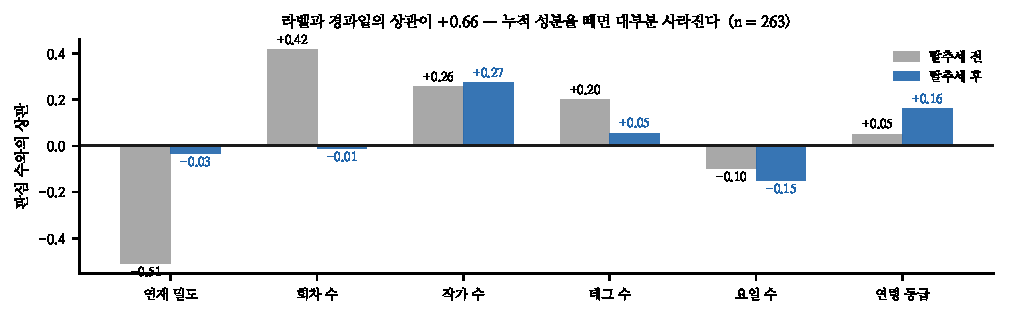
\includegraphics[width=\textwidth]{figs/webtoon.pdf}
\caption{웹툰 변수와 관심 수의 상관. 회색이 탈추세 전, 초록이 후다.}
\end{figure}

관심 수는 연재 시작부터 쌓이므로 경과일과 $+$0.65로 상관된다. 탈추세하면
대부분이 사라진다.

\begin{table}[t]
\centering\tsize
\caption{탈추세 전후 상관.}
\begin{tabular}{lrr}
\toprule
변수 & 탈추세 전 & 후 \\
\midrule
회차 수 & $+$0.43 & \textbf{$-$0.00} \\
연재 밀도 & $-$0.54 & $-$0.11 \\
태그 수 & $+$0.32 & $+$0.11 \\
\textbf{작가 수} & $+$0.22 & \textbf{$+$0.28} \\
연령 등급 & $+$0.01 & $+$0.10 \\
\bottomrule
\end{tabular}
\end{table}

회차 수는 노트 21의 DLC 수와 정확히 같은 구조였다 --- 탈추세 전 $+$0.43이
전부 연재 기간이었고 빼면 0이다. 미리 연재 밀도로 바꿔 두었는데 그것도 $-$0.11에
그친다. 탈추세를 이기고 남은 것은 \textbf{작가 수}뿐이다.

\section{자기 상관이 낮은 배선이 전이가 좋았다}

배선을 세 번 갈았다.

\begin{figure}[t]
\centering
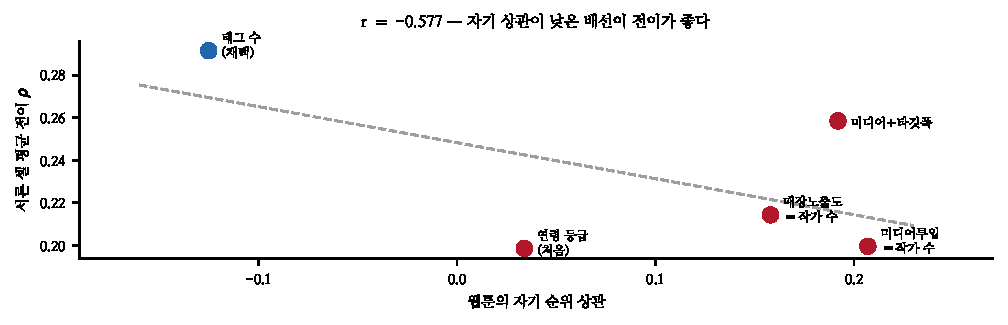
\includegraphics[width=\textwidth]{figs/paradox.pdf}
\caption{웹툰 배선 변형 다섯 개. 가로가 자기 상관, 세로가 전이다.}
\end{figure}

\begin{table}[t]
\centering\tsize
\caption{웹툰 배선 변형.}
\begin{tabular}{lrr}
\toprule
타깃 폭 배선 & 웹툰 자기 $\rho$ & 30셀 평균 \\
\midrule
연령 등급(처음) & $+$0.034 & $+$0.1985 \\
매장 노출도$=$작가 수 & $+$0.158 & $+$0.2143 \\
미디어 투입$=$작가 수 & $+$0.207 & $+$0.1995 \\
미디어$+$타깃 폭$=$태그 & $+$0.192 & $+$0.2585 \\
\textbf{태그 수(채택)} & \textbf{$-$0.125} & \textbf{$+$0.2915} \\
\bottomrule
\end{tabular}
\end{table}

다섯 변형에서 자기 상관과 전이의 상관이 $-$0.72다. \textbf{자기 라벨을 가장
못 맞히는 배선이 남에게 가장 잘 옮겨진다.}

\claimx{노트 40의 상충 법칙이 한 도메인 안에서, 배선을 바꾸는 것만으로 재현된다.
웹툰에서는 자기 순위 상관이 음수인 배선이 최선이었다.}{자기 상관이 음수인데
전이가 좋은 것은 극단이다. 표본이 늘었을 때 부호가 유지되지 않으면 226건의
요동이었던 것이다.}

의미로는 연령 등급이 타깃 폭의 가장 직접적인 측정처럼 보였다 --- 전체 이용가와
성인물은 닿을 수 있는 사람 수가 애초에 다르다. 검정은 태그 수를 골랐다.
노트 28·34·35에 세 번 적은 규칙이 네 번째로 확인된다.

\section{구간은 5\%만 좁아졌다}

\begin{figure}[t]
\centering
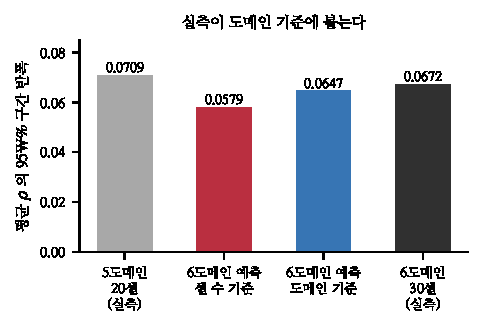
\includegraphics[width=\columnwidth]{figs/narrow.pdf}
\caption{구간 반폭. 실측이 도메인 기준 예측에 붙는다.}
\end{figure}

\begin{table}[t]
\centering\tsize
\caption{도메인 추가의 효과.}
\begin{tabular}{lrrr}
\toprule
& 셀 & 평균 $\rho$ & 구간 반폭 \\
\midrule
5도메인 & 20 & $+$0.3516 & 0.0709 \\
6도메인 & 30 & $+$0.2923 & \textbf{0.0672} \\
\midrule
\multicolumn{2}{l}{셀 수 기준 예측} & & 0.0579 \\
\multicolumn{2}{l}{도메인 수 기준 예측} & & \textbf{0.0647} \\
\bottomrule
\end{tabular}
\end{table}

\claimx{평균 순위 상관의 유효 표본은 셀 수가 아니라 도메인 수다. 셀들이 같은
도메인의 레코드를 공유하므로 붓스트랩 요동이 공통이고, 셀을 늘려도 독립 정보가
그만큼 늘지 않는다.}{일곱째 도메인에서 반폭이 $0.0672\times\sqrt{6/7}=0.0622$
근처가 아니라 셀 기준(0.0549)에 가까우면 이 진단이 틀렸다.}

노트 45는 필요 표본을 \emph{레코드} 기준으로 계산했다. 도메인이 유효 표본이라면
그 계산은 낙관적이었다 --- 알고리즘 급 효과(0.022)를 보려면 반폭 0.011이
필요하고, 도메인 수로는 $6\times(0.0672/0.011)^2\approx220$개가 든다.

\begin{quote}\fontsize{9.5}{11.5}\selectfont
\textbf{절대값 구간으로는 알고리즘 조정을 영원히 검정할 수 없다.} 다만 노트 44가
쓴 \emph{짝지은} 구간은 도메인 공통 요동이 상쇄돼 훨씬 좁다(차이 구간 반폭
0.02--0.04 대 절대값 0.07). 앞으로의 비교는 전부 짝지어야 한다.
\end{quote}

\section{나쁜 도메인은 무엇을 망치나}

평균이 $+$0.3516에서 $+$0.2923으로 떨어졌으니 웹툰이 다른 도메인의 전이를
해쳤나 의심했다. 아니다.

\begin{table}[t]
\centering\tsize
\caption{기존 20셀만 따로 잰 것.}
\begin{tabular}{lr}
\toprule
& 20셀 평균 \\
\midrule
5도메인 & $+$0.3516 \\
6도메인 ($\lambda$ 6도메인 유도) & $+$0.3516 \\
6도메인 ($\lambda$ 5도메인 고정) & $+$0.3516 \\
\bottomrule
\end{tabular}
\end{table}

소수점 넷째 자리까지 같다. \textbf{나쁜 도메인은 다른 셀을 망치지 않고 평균을
희석할 뿐이다.} 평균이 떨어진 것은 웹툰이 낀 10셀이 $+$0.17로 낮기 때문이다.

\paragraph{웹툰은 상충 법칙의 경계에 있다}
웹툰은 자기 상관이 최저인데 출처로서도 최저다($-$0.18, 태그 배선 전 기준).
노트 40의 법칙대로면 자기 상관이 낮을수록 출처로 좋아야 한다. 어긋나는 이유는
\textbf{자기 상관이 낮은 데 두 가지 이유가 있기} 때문이다 --- 축이 일반적이어서
낮은 것과 축이 무효라서 낮은 것. 앞의 것은 출처로 좋고 뒤의 것은 아무 쓸모가
없다. 다섯 도메인은 모두 앞쪽이었고 웹툰의 첫 배선은 뒤쪽이었다.

\section{한계}

\begin{itemize}[leftmargin=1.1em,itemsep=0.15em]
\item 웹툰 226건은 목표(500)의 절반이고 완결작이 거의 없다. 연재 중인 작품만
      있으면 관심 수가 아직 쌓이는 중이라 경과시간 편향이 크다.
\item 반폭 스케일링을 두 점(5, 6도메인)으로만 봤다. 일곱째가 필요하다.
\item 웹툰 배선 변형 다섯 개에서 최댓값을 골랐다. 짝지은 구간을 붙이지 않았다.
\item 웹툰 매장 노출도는 SD 0.08로 상수 강등 문턱을 겨우 넘는다. 작가 중복이
      적어 사실상 요일 수만 들어 있다.
\item 관심 수를 주당 획득률로 나눠 봤지만 탈추세 후에는 같은 값이 된다
      (log 공간에서 선형 이동이라 흡수된다). 라벨 선택이 문제가 아니었다.
\end{itemize}

\section{다음}

\begin{enumerate}[leftmargin=1.3em,itemsep=0.15em]
\item 웹툰 완결작 확보 --- 연재 중 편향을 줄인다.
\item 모든 비교를 짝지은 구간으로 --- 절대값 구간은 판정에 쓸 수 없다.
\item 웹툰 배선에 짝지은 구간을 붙인다. 태그 수 채택이 잡음일 수 있다.
\item 일곱째 도메인 --- 반폭 스케일링을 세 점으로.
\end{enumerate}

\vspace{0.6em}
\hrule height 0.3pt
\vspace{0.5em}
{\footnotesize
\textbf{참고문헌}\\[0.3em]
Efron, B., Tibshirani, R. J. (1993). \emph{An Introduction to the Bootstrap}.
Chapman \& Hall.\\[0.15em]
Kish, L. (1965). \emph{Survey Sampling}. Wiley. (군집 표본의 유효 표본 크기)\\[0.15em]
Kaufman, S., Rosset, S., Perlich, C. (2012). Leakage in data mining.
\emph{ACM TKDD}, 6(4), 1--21.\\[0.15em]
Standley, T. et al. (2020). Which tasks should be learned together in multi-task
learning? \emph{ICML}, 9120--9132.\\[0.15em]
Ben-David, S. et al. (2010). A theory of learning from different domains.
\emph{Machine Learning}, 79(1--2), 151--175.
}

\end{document}
